\documentclass{article}
\usepackage{parskip}
\usepackage{geometry}
\usepackage{amsmath}
\usepackage{graphicx}
\usepackage{amssymb}
\geometry{letterpaper, margin=1in}

\begin{document}

\title{\textbf{Airfoil Selection - Iteration 3}}
\author{Stephanie Jou}
\date{September 20th, 2020}
\maketitle

After the Spring 2020 semester, the manufacturing team for the Open UAS was created. After several discussions in the design team, it was reached to the conclusion that the airfoil would be changed as well as the tail of the UAS for the new iteration. This would leave the current fuselage design unchanged. Because this decision regarding the airfoil was reached, several airfoils were analyzed. In this document, information regarding the decisions and steps made are given.

\section{Choosing New Airfoils}
During the first weeks of the Fall 2020 semester, team members made research on different airfoils and proposed them to be considered for the new iteration. In total, four airfoils were analyzed. The S1223 was chosen since in the previous analysis made, this airfoil got the best evaluation. However, this airfoil was not chosen since it was considered troublesome to manufacture given its cambered shape. With the formation of the new manufacturing team, this airfoil was considered once again. The current airfoil, Clark Y, was analyzed again for comparison to the other proposed airfoils. The last two airfoils suggested were the NACA 23012 and NACA 23015. These were proposed based on the thickness value in comparison to model planes currently owned.

\section{Completing XFLR5 Analyses}
As with previous iterations, XFLR5 was used to analyze the airfoils. The Reynolds number used was 170,000. This was calculated with a speed of 20 m/s (about 44.7 mph), chord length of about 0.4 ft (0.1245 m) and a kinematic viscosity of 1.4657x10\textsuperscript{-5}m\textsuperscript{2}/s. The Mach number obtained was of 0.059. A Ncrit value of 9 was used as well as a Type 1 analysis. The data returned ranged from -5 degrees to 20 degrees. The information was all exported into several csv files where specific graphs and information were extracted. 

\section{Data Analysis}
For each of the airfoils, the following graphs were done: $Cl$ vs $\alpha$, $Cl/Cd$ vs $\alpha$, $Cl$ vs $Cd$ . From these graphs, the following information was extracted: Cl\textsubscript{0}, Cl\textsubscript{max}, stall angle, Cd\textsubscript{min}, and maximum efficiency E\textsubscript{max}.\\

For Cl\textsubscript{0}, the value of lift at a 0 degree angle of attack was extracted from the $Cl$ vs $\alpha$ data. For the maximum lift coefficient, the maximum lift value was extracted from the data. For the stall angle, the $Cl$ vs $\alpha$ graph was used. With this graph, the approximate angle at which the linear tendency stops was used. For the Cd\textsubscript{min}, the $Cl$ vs $Cd$ graph was used with the Cd value when Cl equaled 0 was extracted. For the maximum efficiency, the $Cl/Cd$ vs $\alpha$ graph was used. This maximum value for the Cl/Cd was extracted. The results will be shown in a table format comparing the 4 airfoils later in this document.

\section{Graphs Obtained}
\subsection{NACA 23012}
\begin{figure}[!h]
\begin{center}
	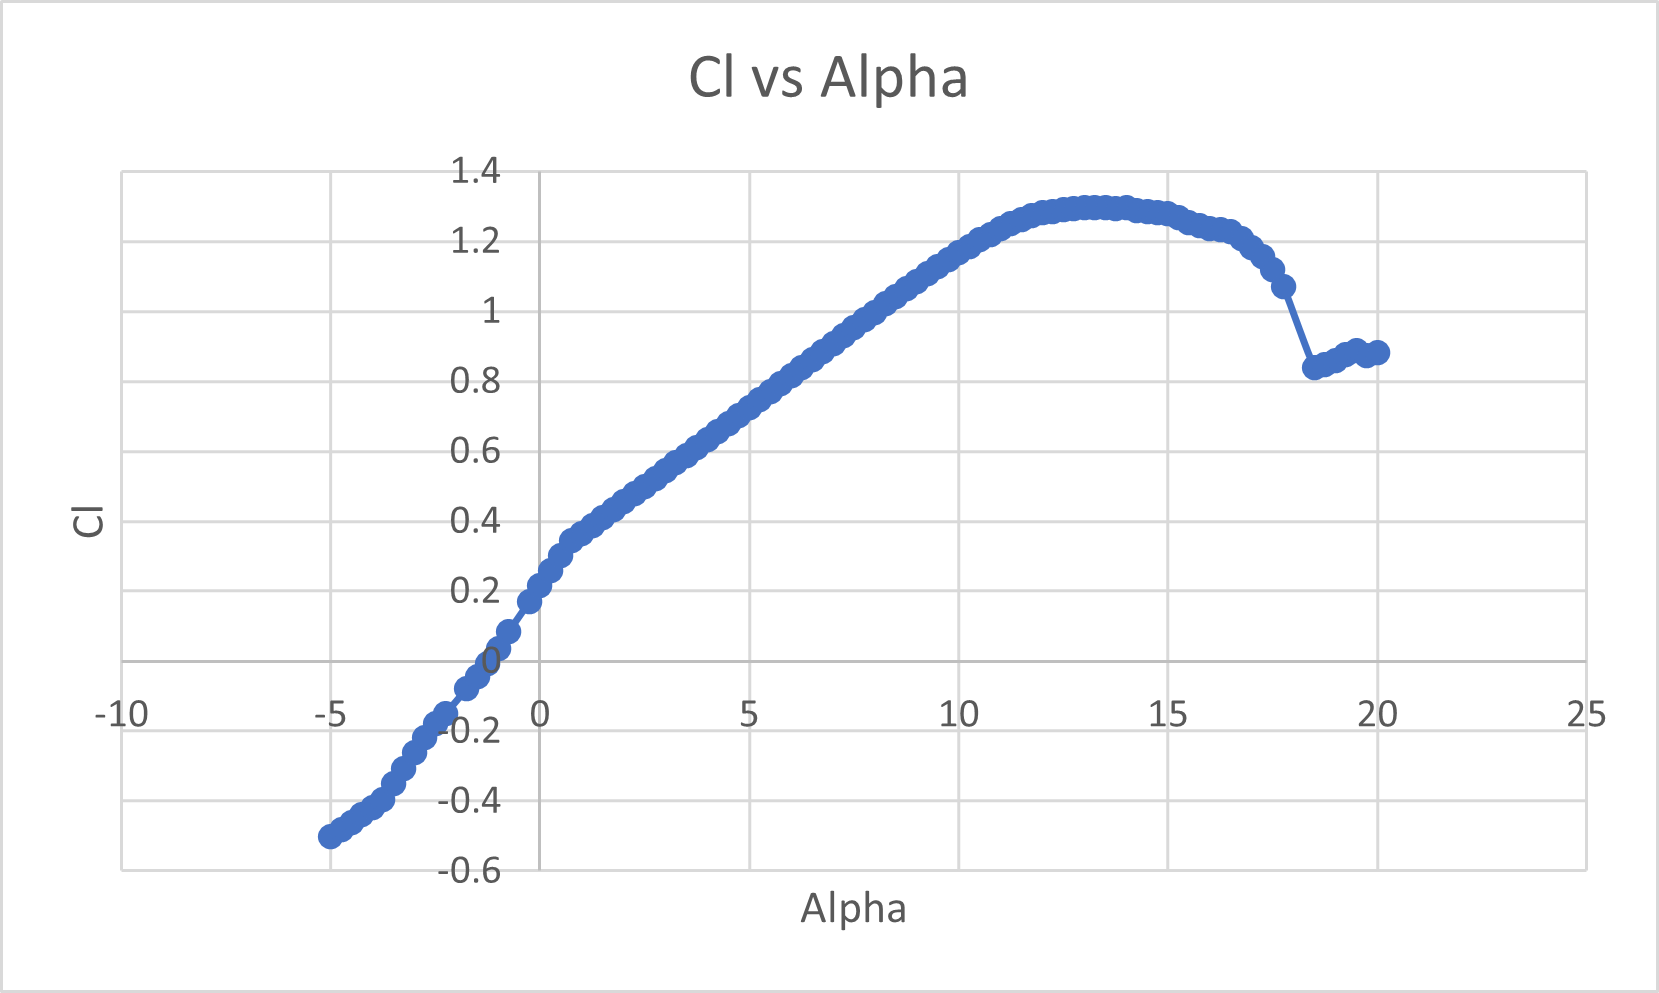
\includegraphics[scale=0.7]{NACA 23012 Clalpha.png}
	\caption{NACA 23012 $Cl$ vs $\alpha$}
	\label{Figure1:}
\end{center}
\end{figure}

\begin{figure}[!h]
\begin{center}
	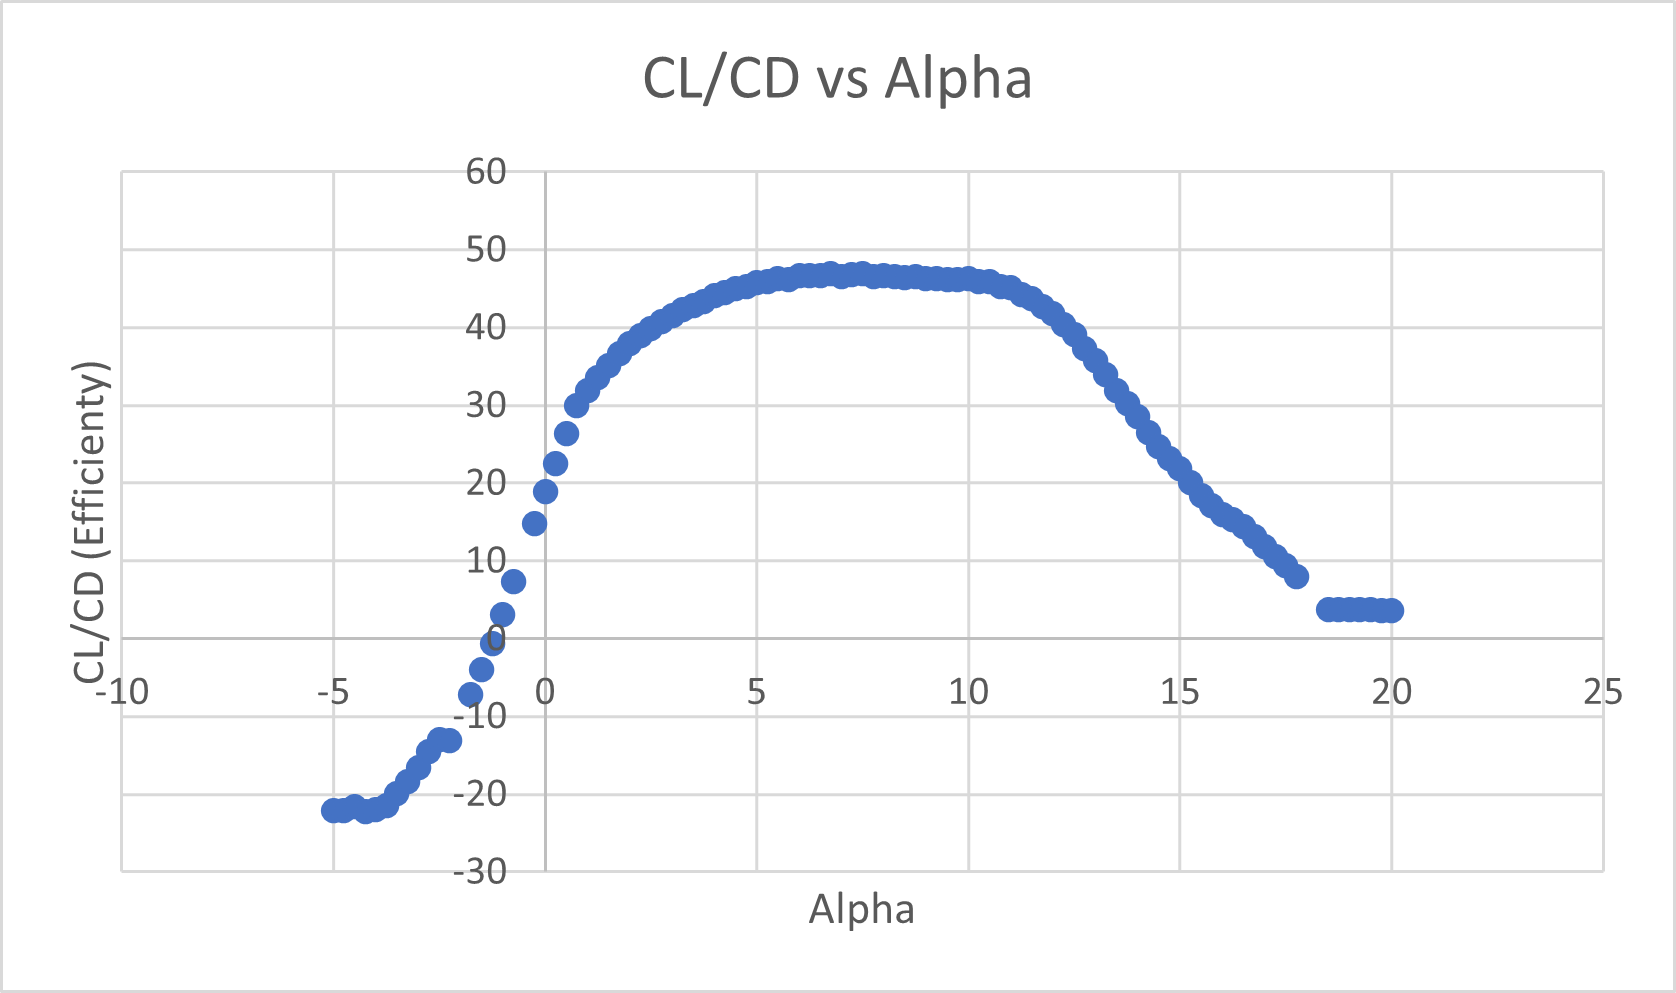
\includegraphics[scale=0.7]{NACA 23012 Efficiencyalpha.png}
	\caption{NACA 23012 $Cl/Cd$ vs $\alpha$}
	\label{Figure2:}
\end{center}
\end{figure}

\begin{figure}[!h]
\begin{center}
	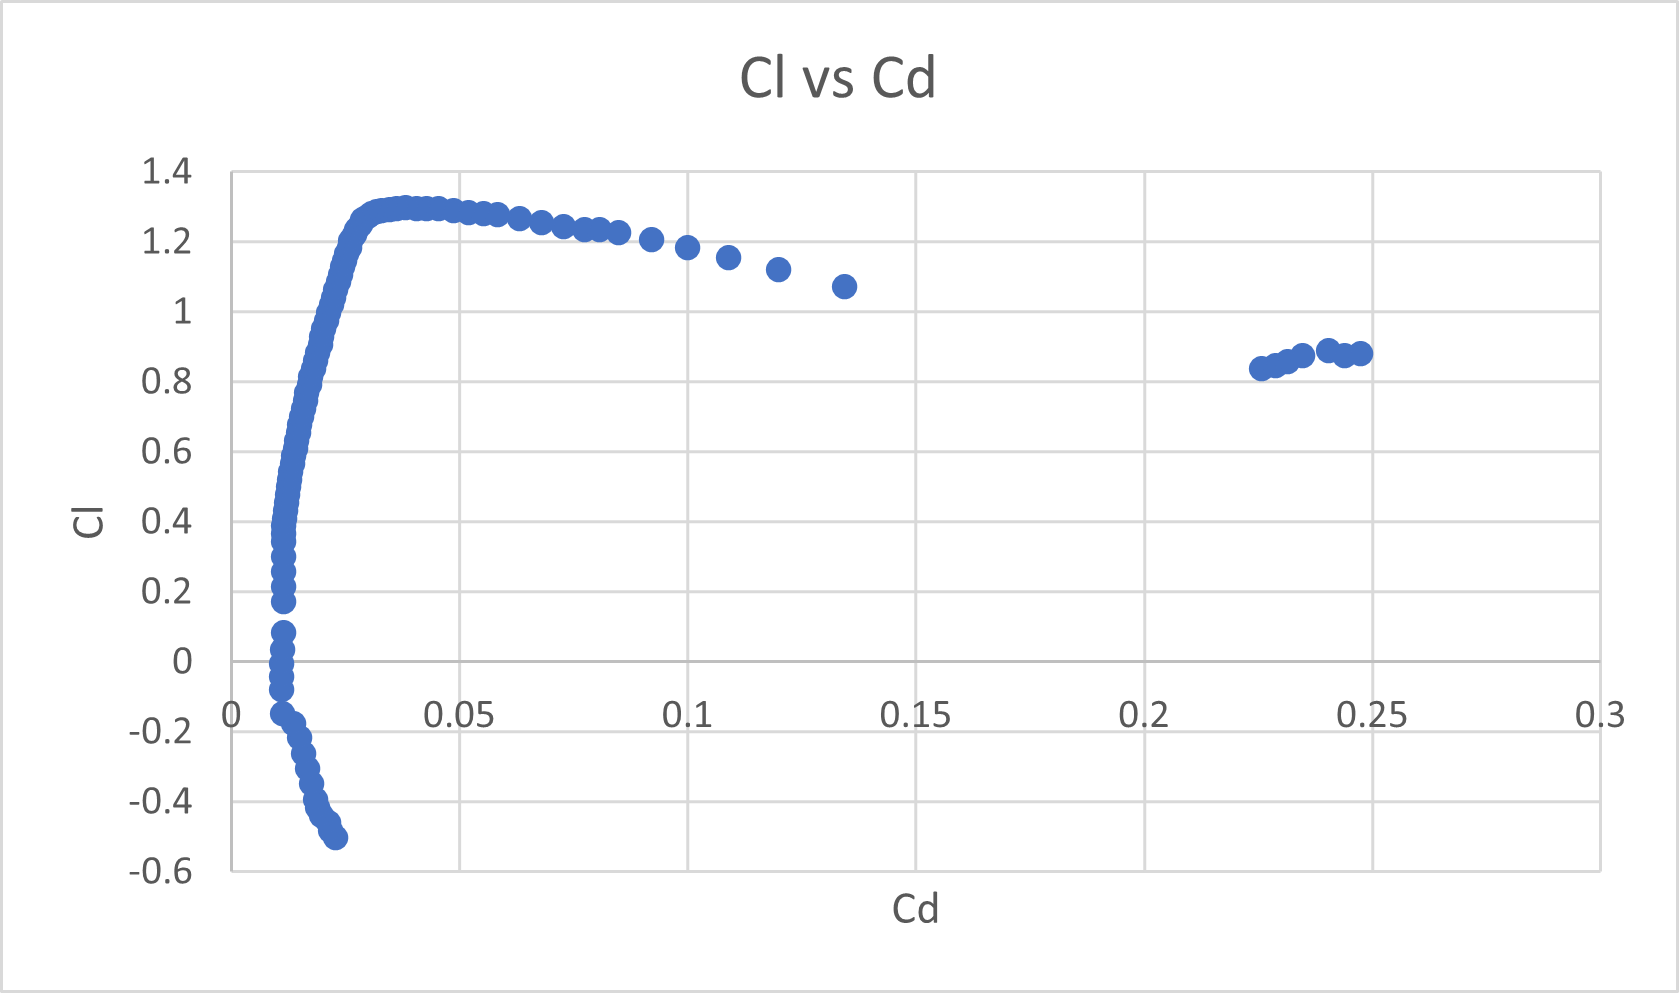
\includegraphics[scale=0.7]{NACA 23012 ClCd.png}
	\caption{NACA 23012 $Cl$ vs $Cd$}
	\label{Figure3:}
\end{center}
\end{figure}

\newpage
\subsection{NACA 23015}
\begin{figure}[!h]
\begin{center}
	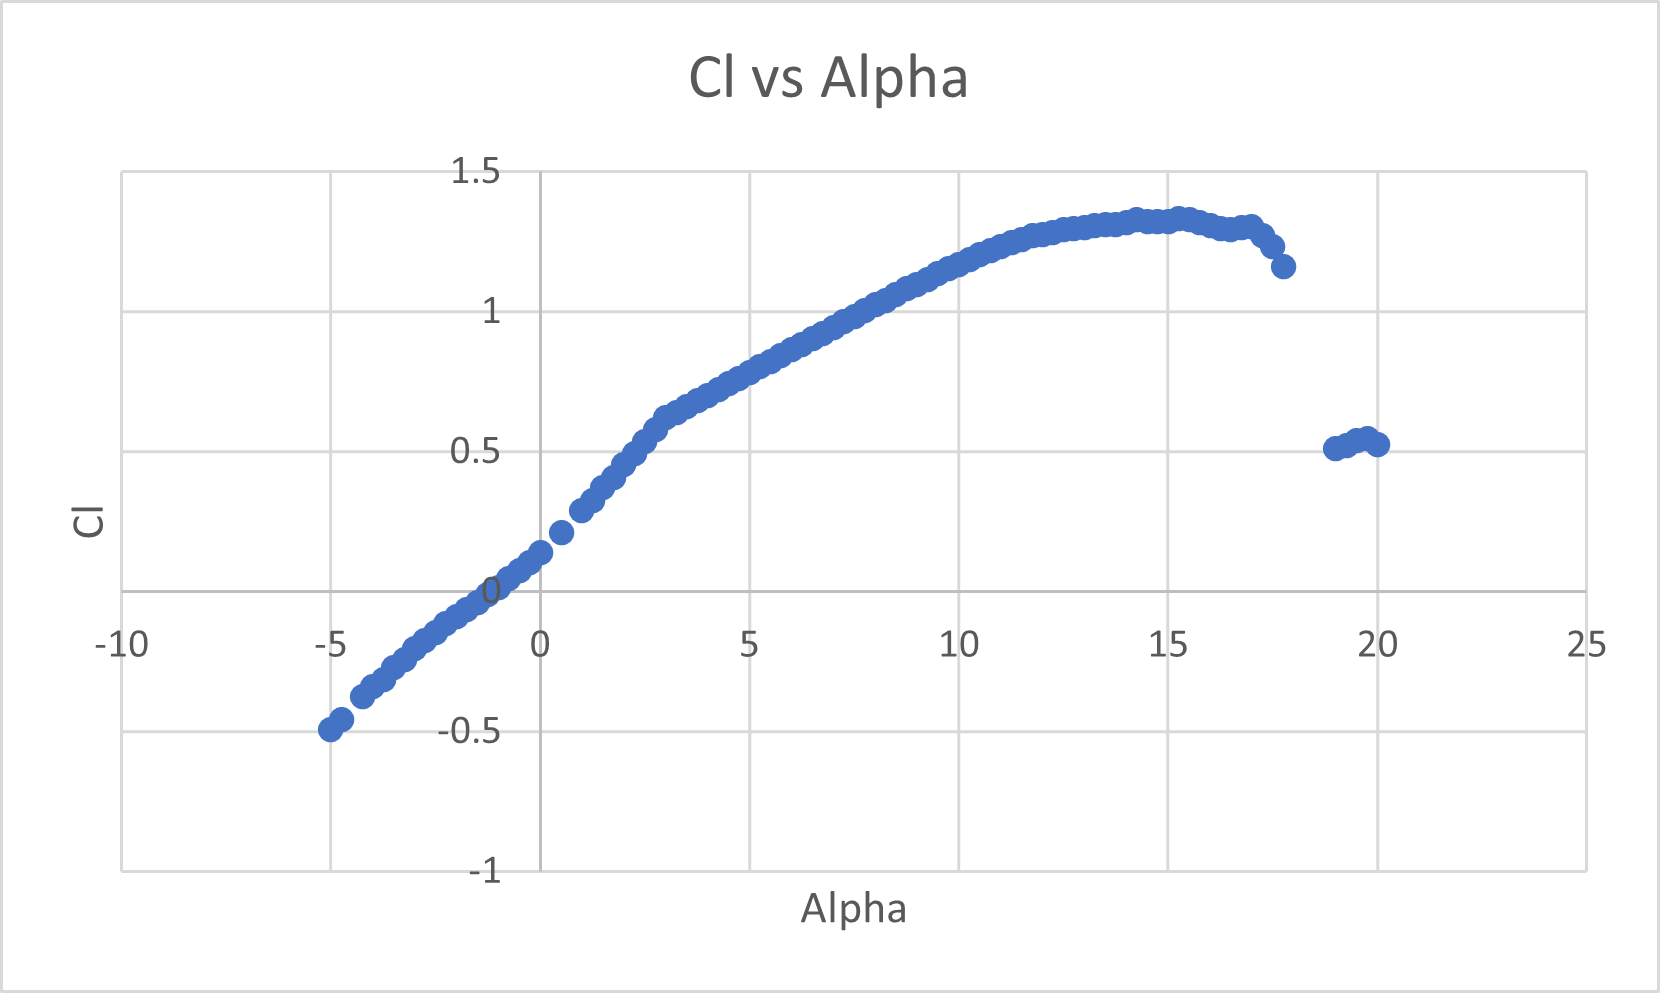
\includegraphics[scale=0.7]{NACA 23015 Clalpha.png}
	\caption{NACA 23015 $Cl$ vs $\alpha$}
	\label{Figure4:}
\end{center}
\end{figure}

\begin{figure}[!h]
\begin{center}
	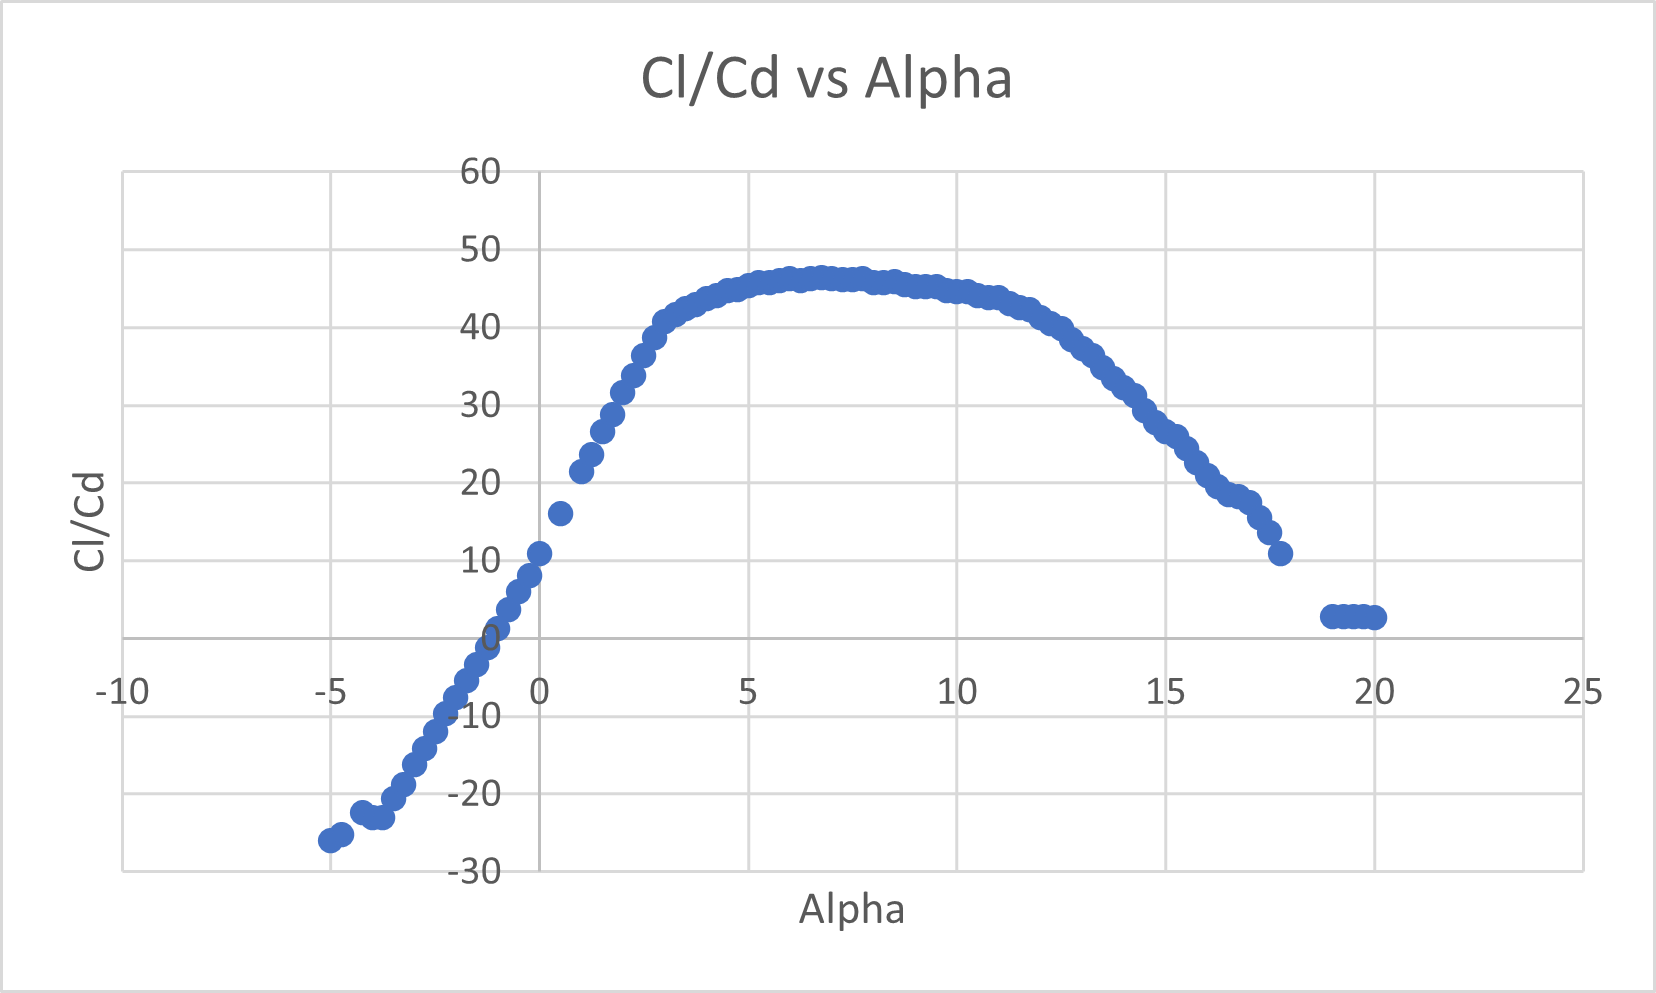
\includegraphics[scale=0.7]{NACA 23015 Efficiencyalpha.png}
	\caption{NACA 23015 $Cl/Cd$ vs $\alpha$}
	\label{Figure5:}
\end{center}
\end{figure}

\begin{figure}[!h]
\begin{center}
	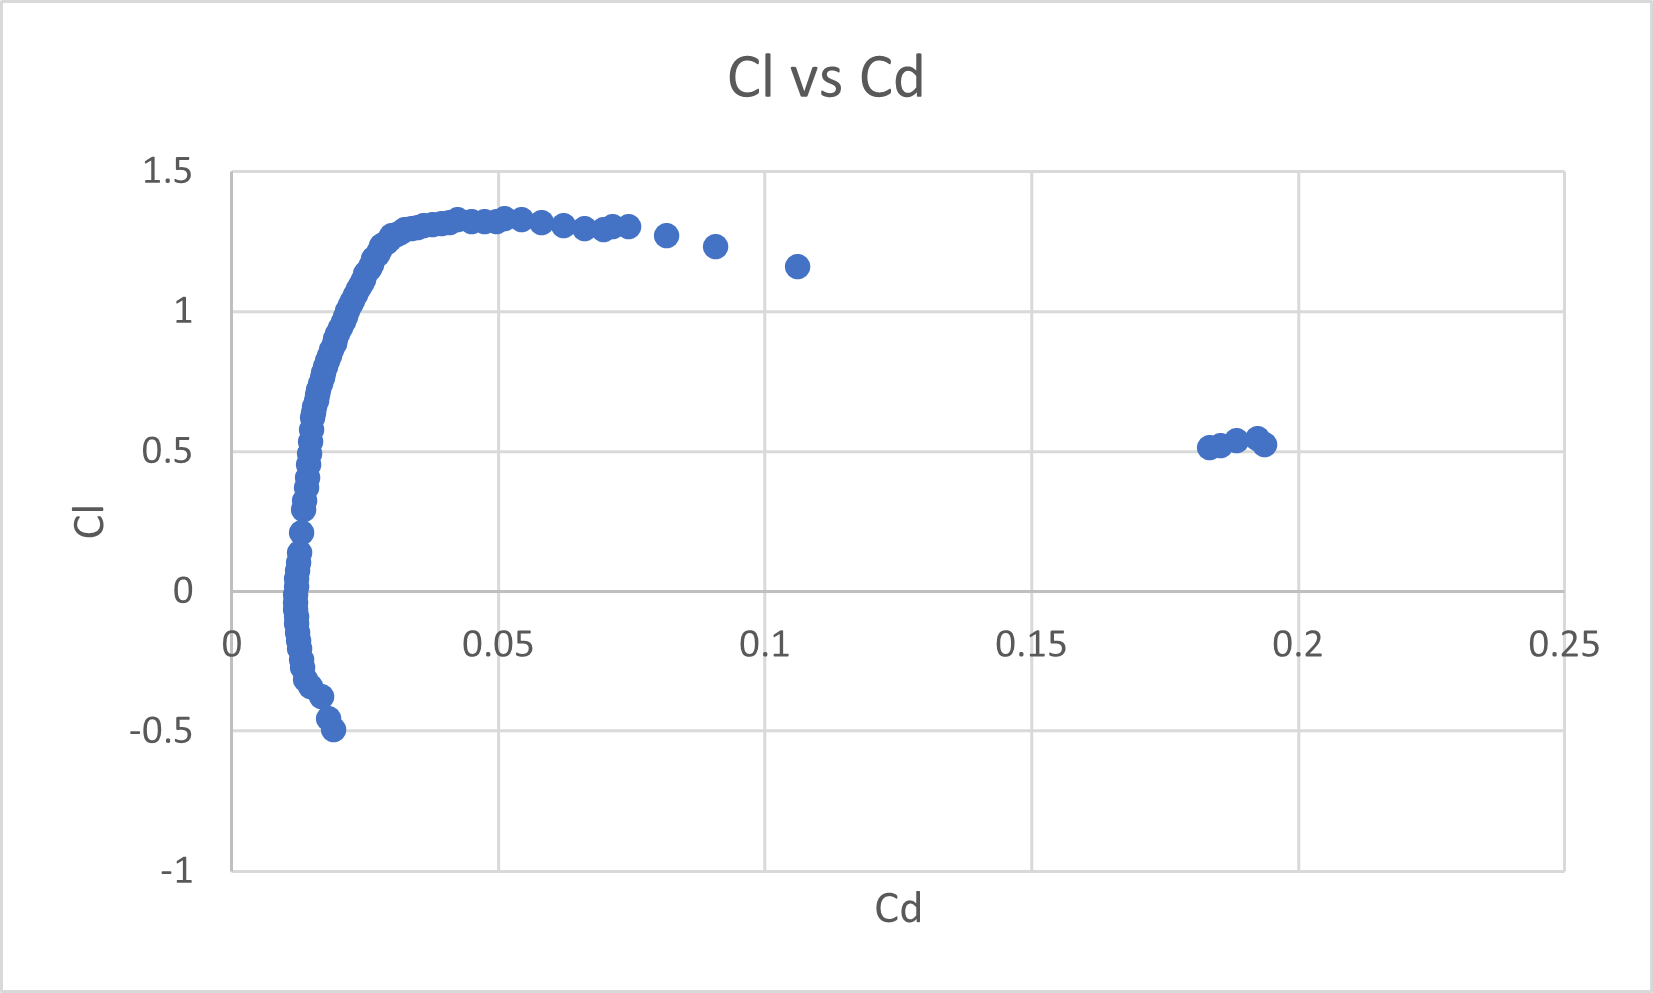
\includegraphics[scale=0.7]{NACA 23015 ClCd.png}
	\caption{NACA 23015 $Cl$ vs $Cd$}
	\label{Figure6:}
\end{center}
\end{figure}

\newpage
\subsection{S1223}
\begin{figure}[!h]
\begin{center}
	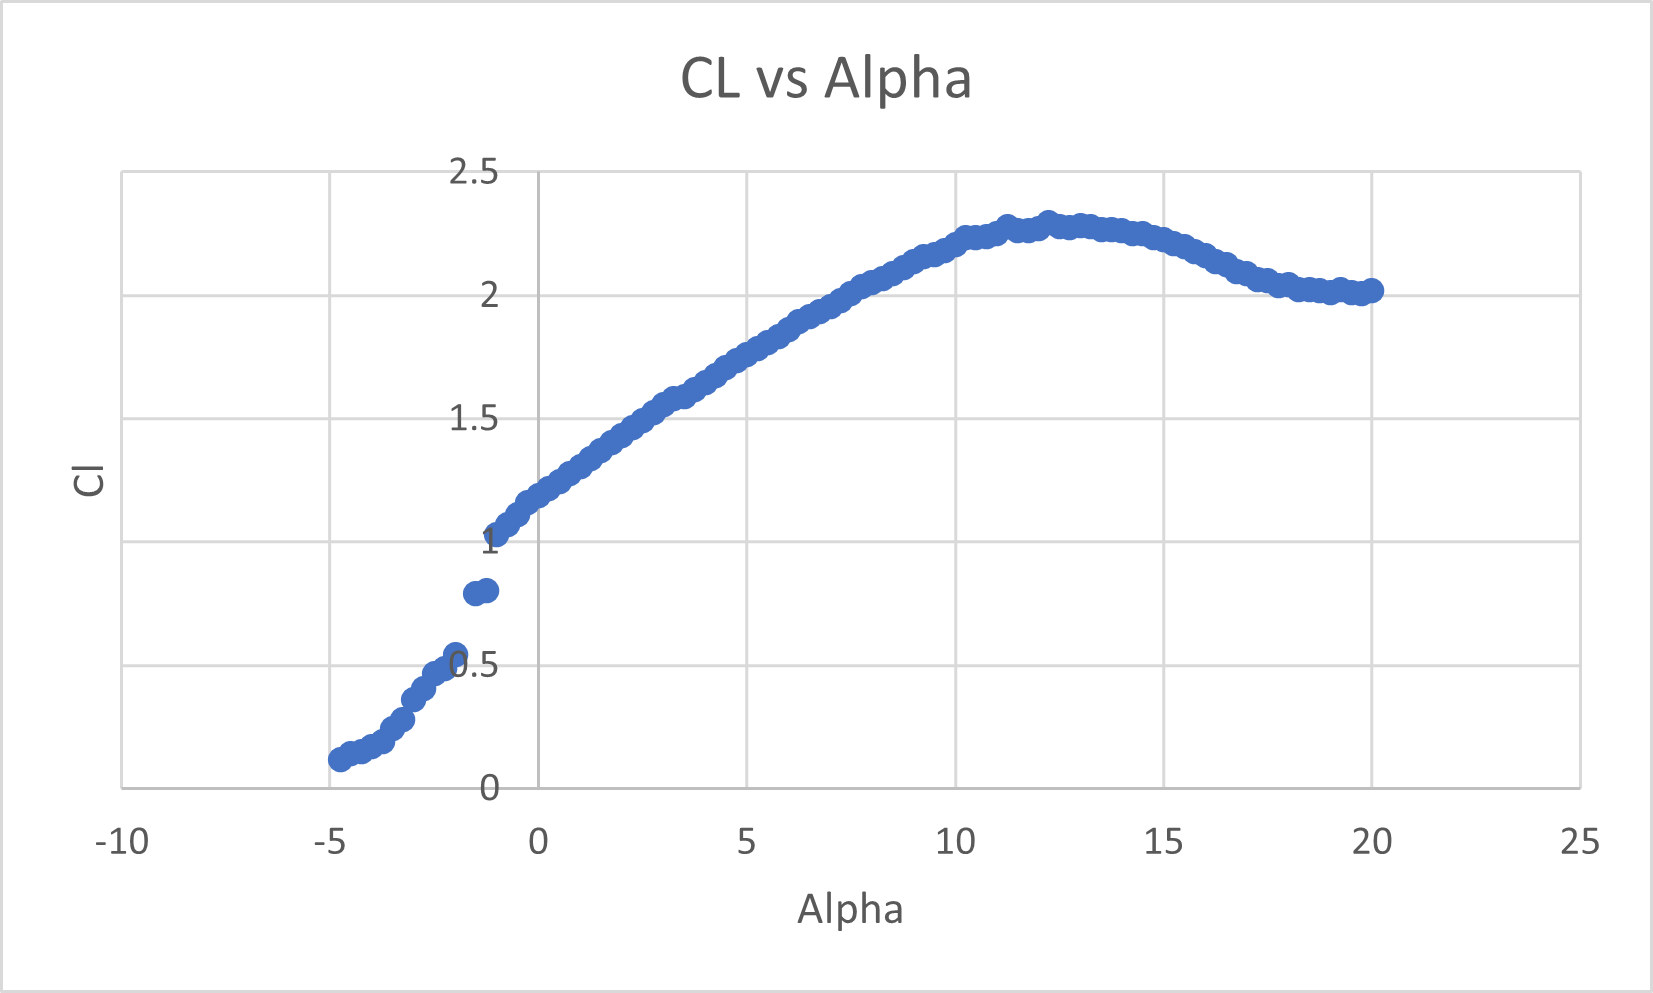
\includegraphics[scale=0.7]{S1223 Clalpha.png}
	\caption{S1223 $Cl$ vs $\alpha$}
	\label{Figure7:}
\end{center}
\end{figure}

\begin{figure}[!h]
\begin{center}
	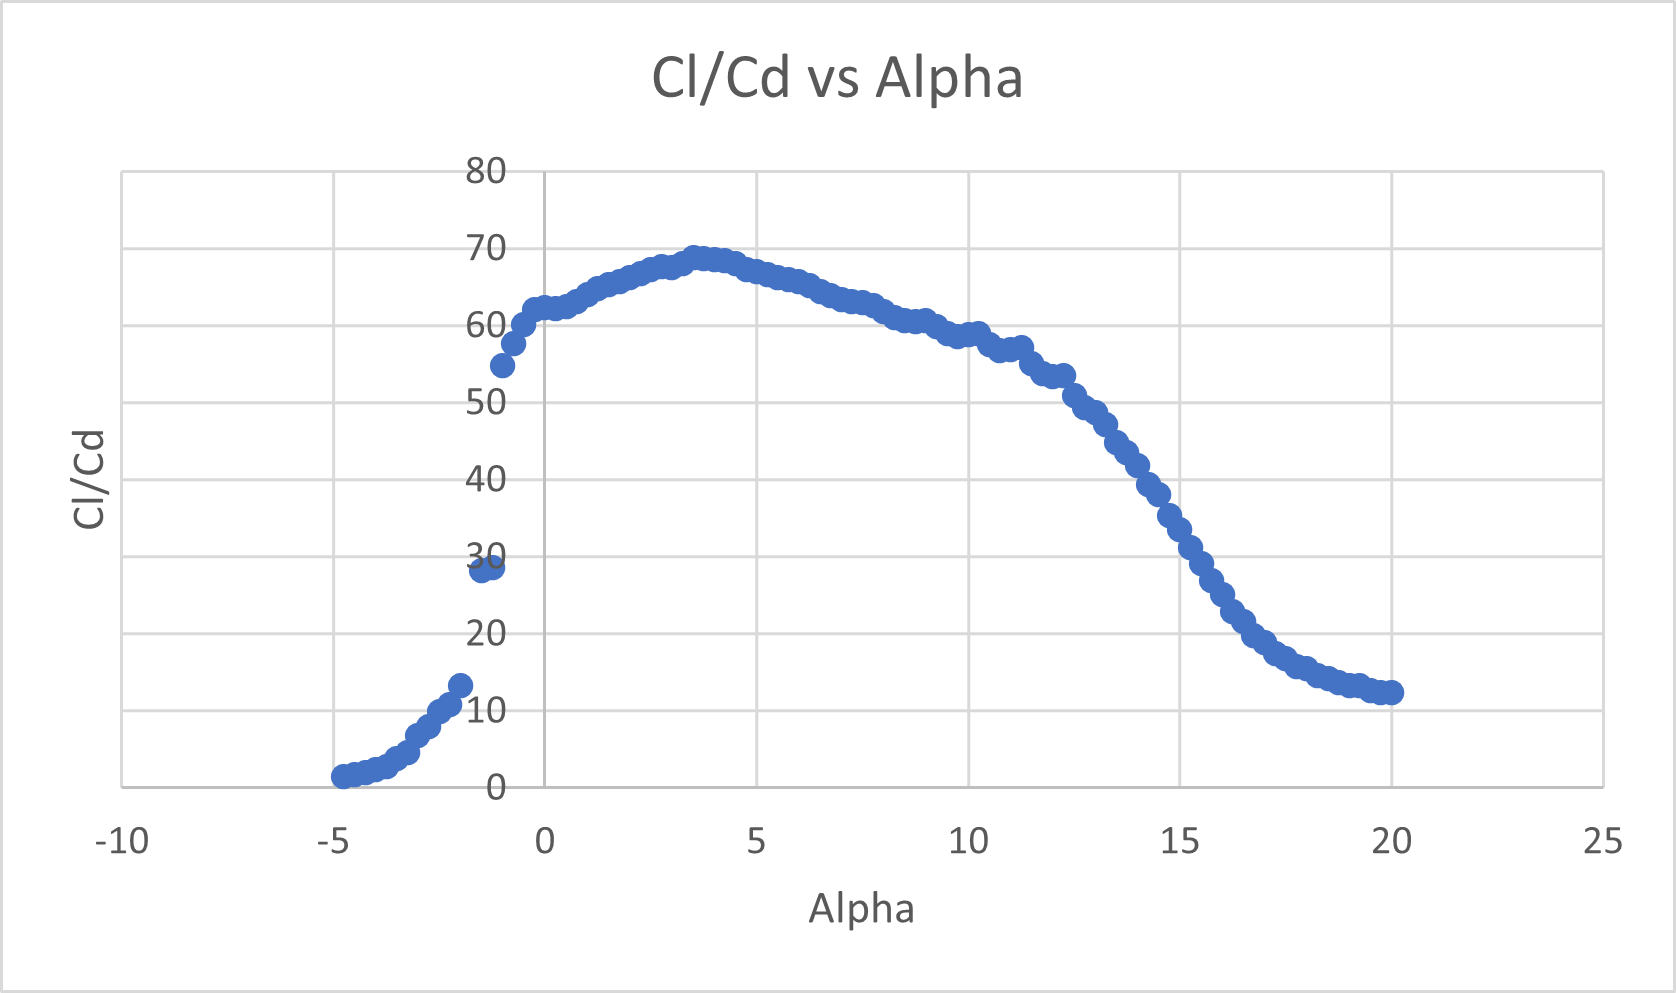
\includegraphics[scale=0.7]{S1223 Efficiencyalpha.png}
	\caption{S1223 $Cl/Cd$ vs $\alpha$}
	\label{Figure8:}
\end{center}
\end{figure}

\begin{figure}[!h]
\begin{center}
	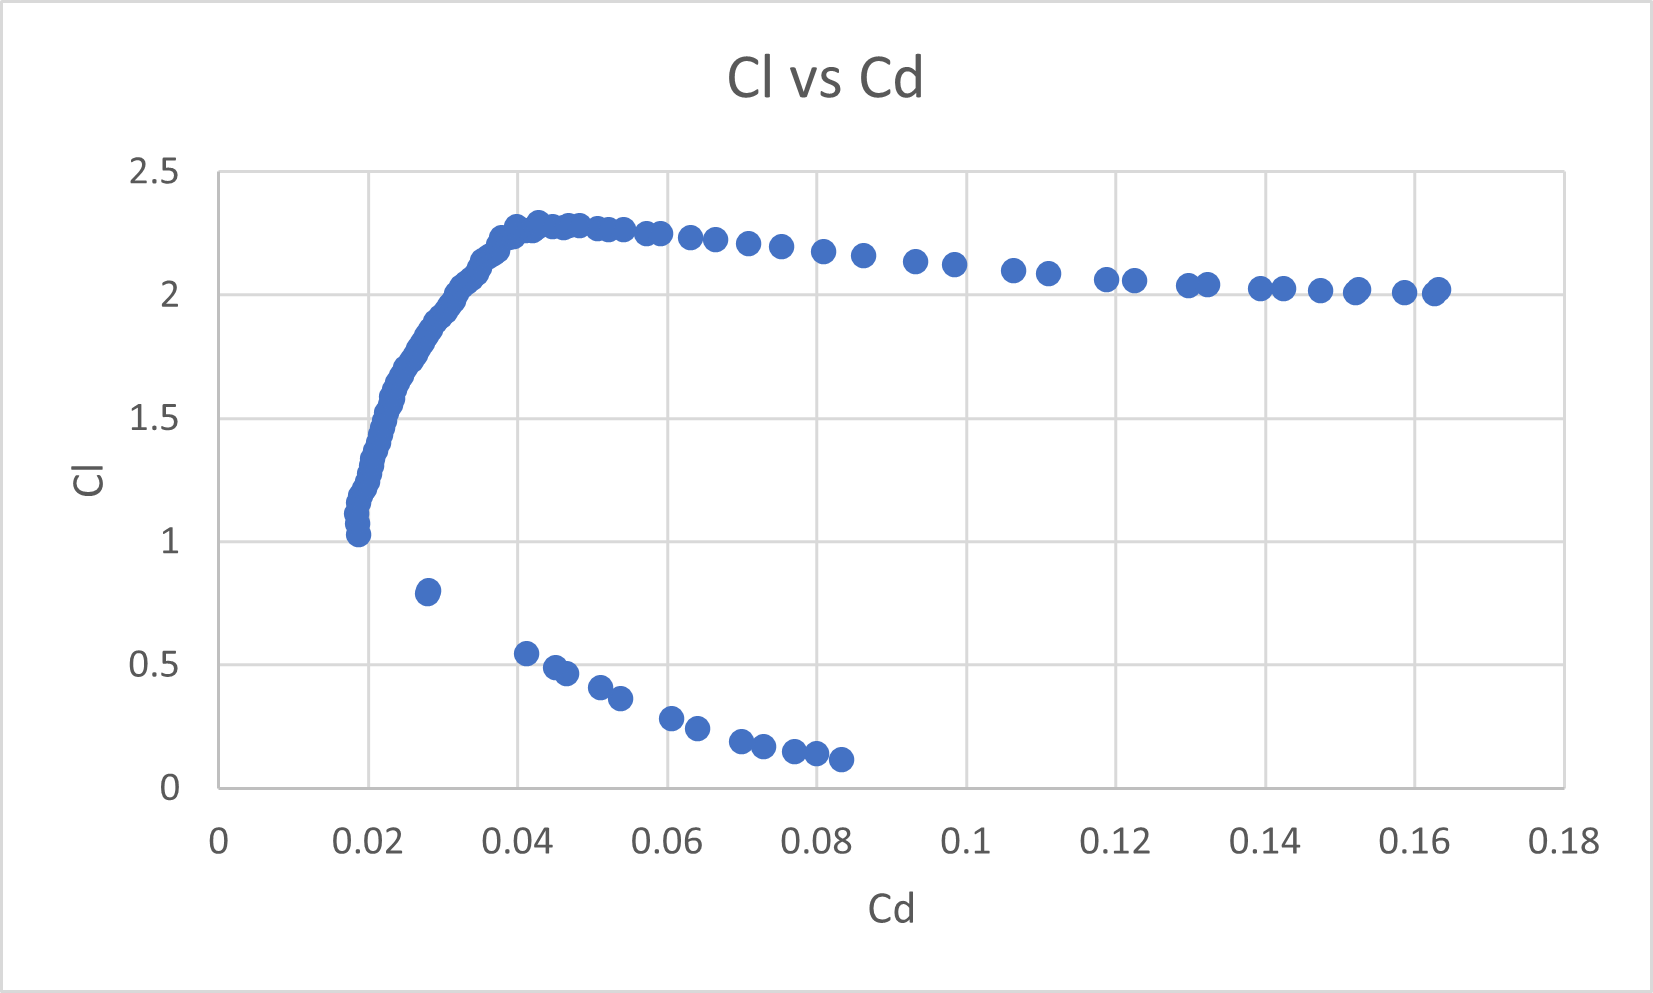
\includegraphics[scale=0.7]{S1223 ClCd.png}
	\caption{S1223 $Cl$ vs $Cd$}
	\label{Figure9:}
\end{center}
\end{figure}

\newpage
\subsection{Clark Y}
\begin{figure}[!h]
\begin{center}
	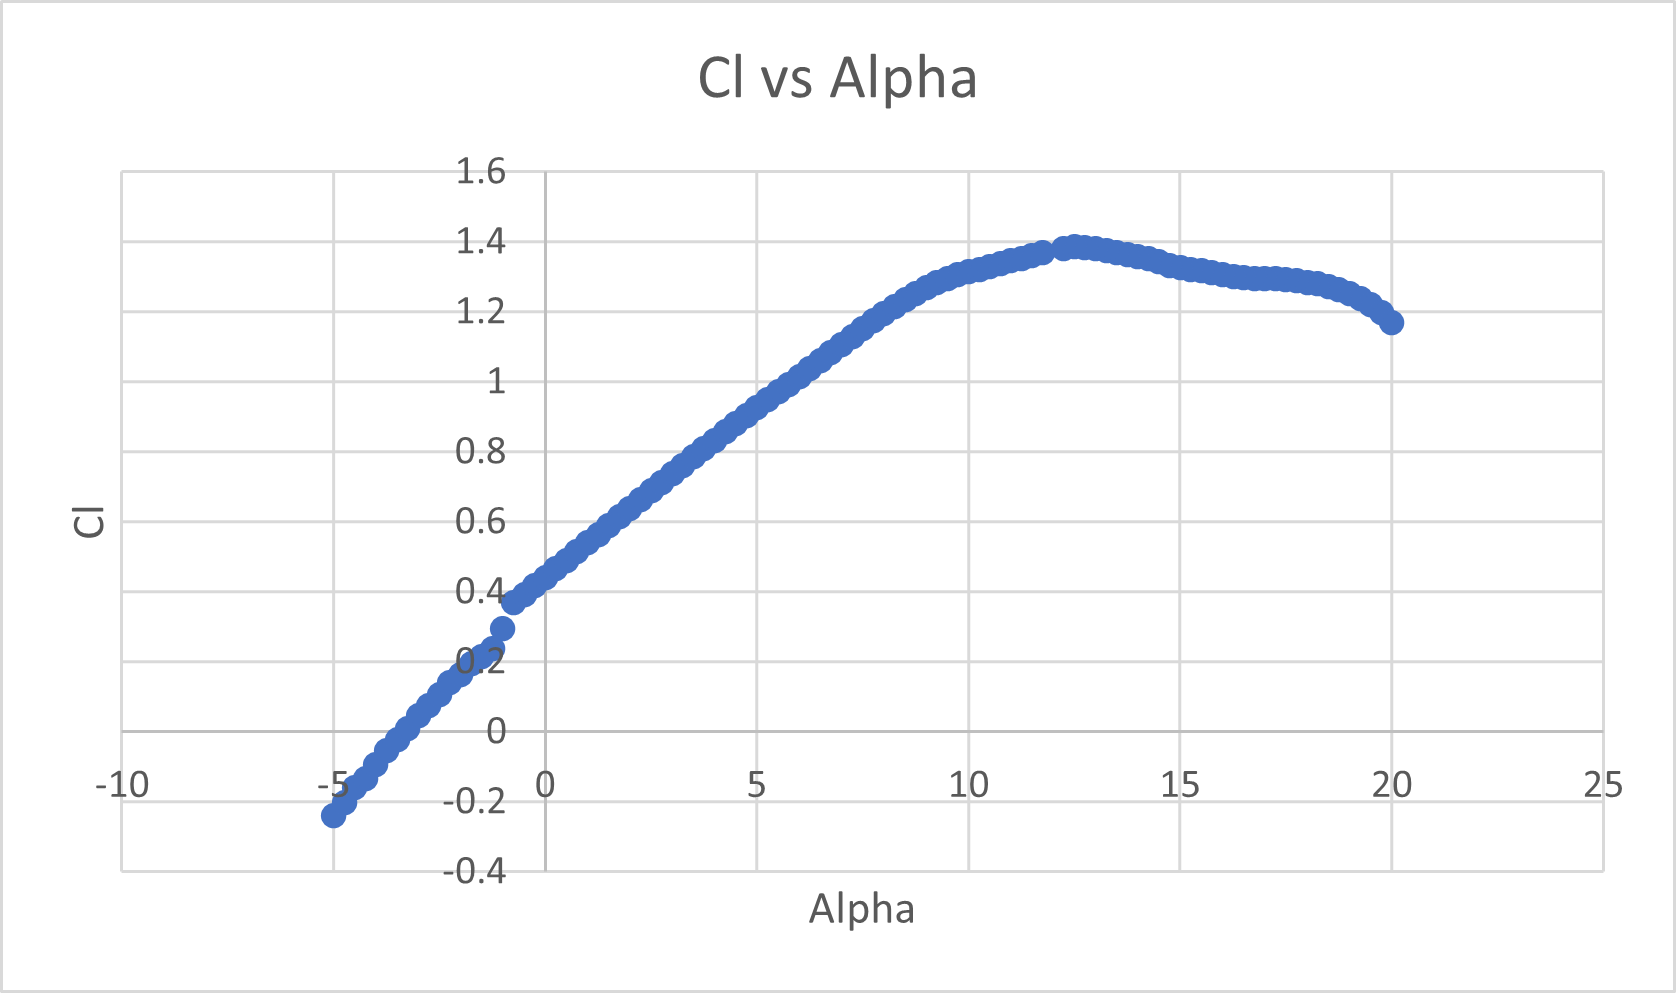
\includegraphics[scale=0.7]{ClarkY Clalpha.png}
	\caption{Clark Y $Cl$ vs $\alpha$}
	\label{Figure10:}
\end{center}
\end{figure}

\begin{figure}[!h]
\begin{center}
	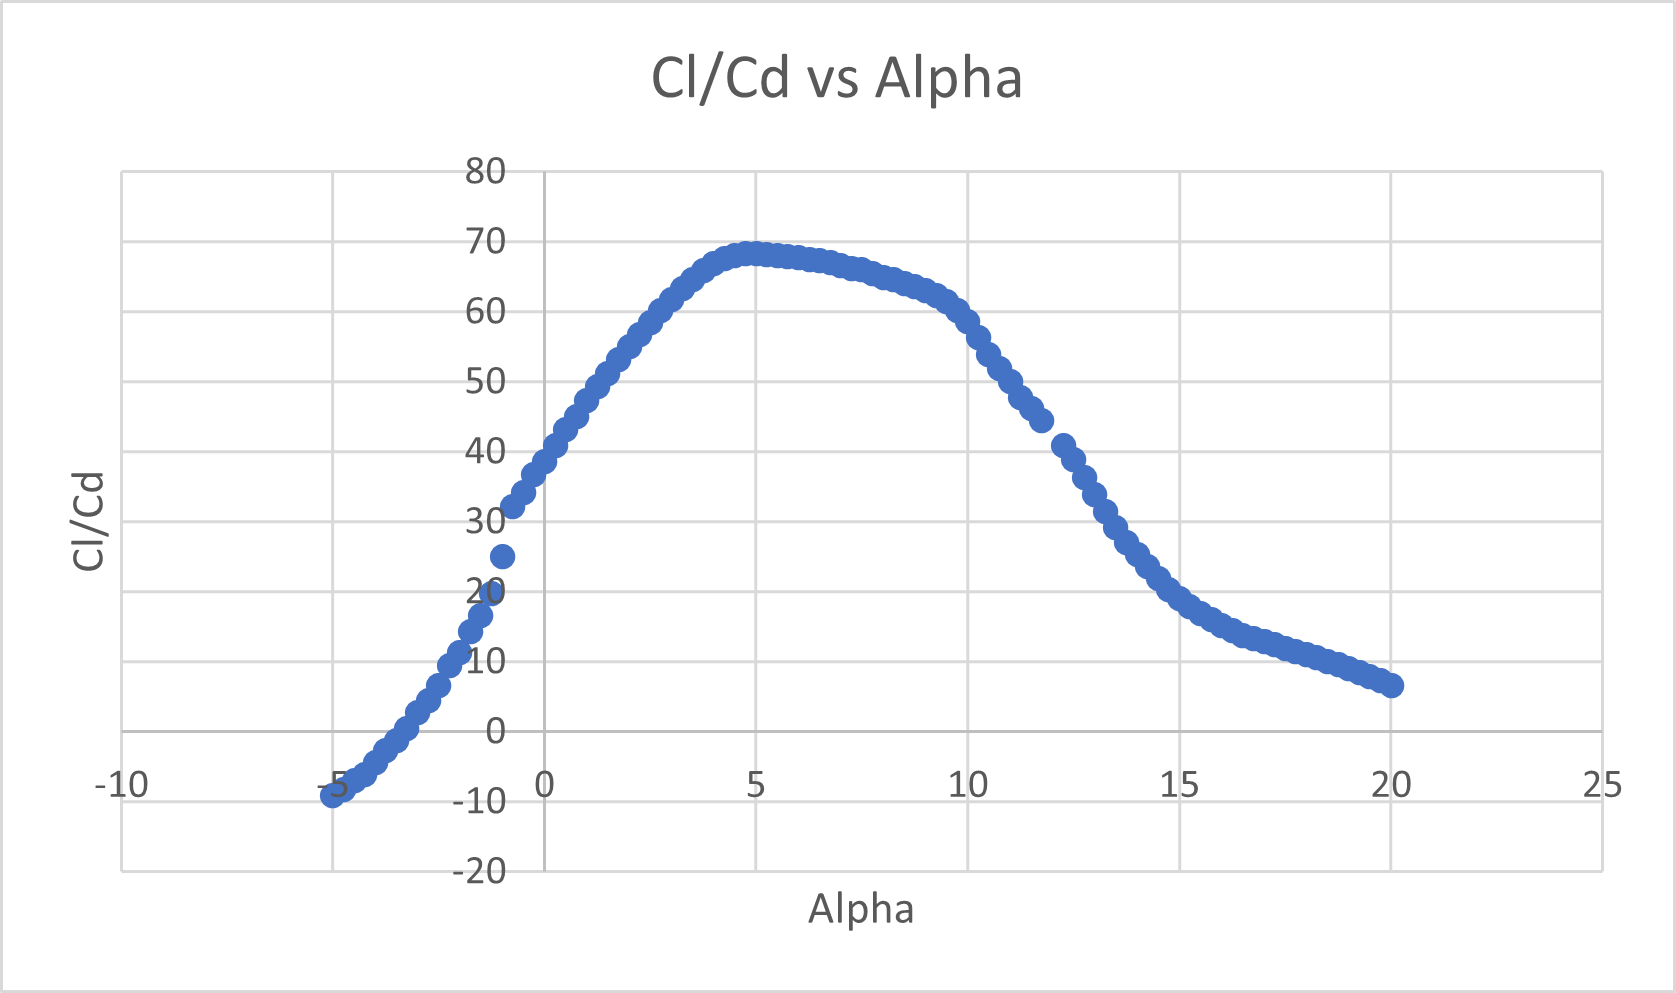
\includegraphics[scale=0.7]{ClarkY Efficiencyalpha.png}
	\caption{Clark Y $Cl/Cd$ vs $\alpha$}
	\label{Figure11:}
\end{center}
\end{figure}

\begin{figure}[!h]
\begin{center}
	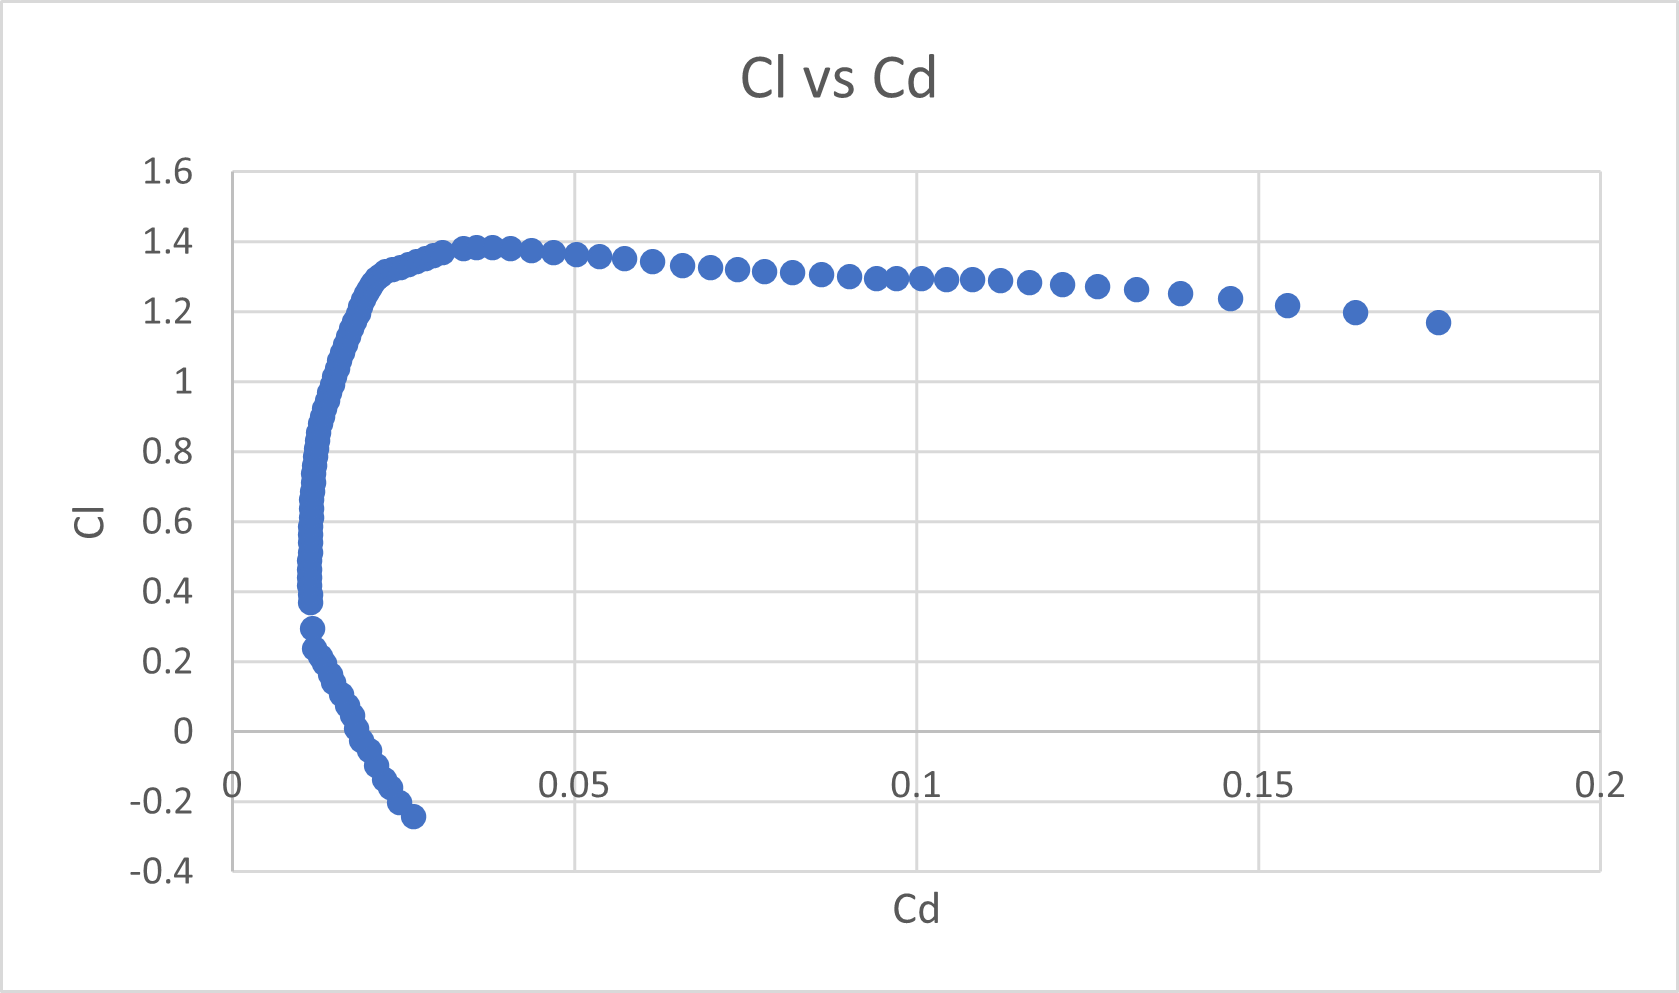
\includegraphics[scale=0.7]{ClarkY ClCd.png}
	\caption{Clark Y $Cl$ vs $Cd$}
	\label{Figure12:}
\end{center}
\end{figure}

\newpage
\section{Results Obtained}
\begin{tabular}[pos]{| c | c | c | c | c |}
\hline
Parameter & NACA 23012 & NACA 23015 & S1223 & Clark Y\\ \hline
$Cl_{0}$ & 0.2163 & 0.1386 & 1.187 & 0.4399   \\ \hline
$Cl_{max}$  & 1.2969 & 1.3317 & 2.2938 & 1.3853 \\ \hline
$\alpha_{stall}$ & 10.75 & 10.25 & 9.5 & 9 \\ \hline
$Cd_{min}$ & 0.01122 & 0.01208 & 0.08337 & 0.01823 \\ \hline
$E_{max}$ & 46.925 & 46.433 & 68.830 & 68.280 \\ \hline
\end{tabular}

\section{Weighing of Results}
Simiarly to the previous iteration, the results were weighed. The same scale as the one done for the previous iteration was used. For each airfoil, its parameter is rated as 1st, 2nd, 3rd, or 4th. If the airfoil gets 1st for a parameter, 4 points is given. If it gets 2nd, 3 points are given. If it gets 3rd, 2 points are given. If it gets 4th, 1 point is given. The results are shown below.\\
\begin{tabular}[pos]{| c | c | c | c | c | c | c |}
\hline
Parameter & Evaluation & NACA 23012 & NACA 23015 & S1223 & Clark Y & Multiplier \\ \hline
$Cl_{0}$ & Closest to cruise better & 3rd & 4th & 1st & 2nd & 1.2  \\ \hline
$Cl_{max}$ & Highest is the best & 4th & 3rd & 1st & 2nd & 1.25 \\ \hline
$\alpha_{stall}$ & Highest is the best & 1th & 2nd & 3rd & 4th & 1.15 \\ \hline
$Cd_{min}$ & Lowest is the best & 1st & 2nd & 4th & 3rd & 1.15 \\ \hline
$E_{max}$ & Highest is the best & 3rd & 4th & 1st & 2nd & 1.25  \\ \hline
Total Points & & \textbf{15.35} & \textbf{11.85} & \textbf{18.25} & \textbf{14.55} & \\ \hline
\end{tabular}

\section{Analysis of Results}
Based on the table shown above, the NACA 23012 and the S1223 airfoils are better than the Clark Y. At this point, no final decision based on manufacturability has been made between the 2 airfoils so CAD models have been done of both airfoils and separate assemblies have been made for each airfoil. Once a final decision is made, this document will be updated.

\section{References and Documents Used}
[1] Airfoil Selection - Iteration 2 by Abigail Gries


\end{document}